\subsection{Explicit Fusion Algorithm Selection}

        An explicit fusion algorithm is required to intelligently combine the thermal and radar probability maps, \(\mathcal{P}_\text{thermal}(x, y)\) and \(\mathcal{P}_\text{radar}(x, y)\), respectively, into a final probability map, \(\mathcal{P}_\text{fused}(x, y)\), over the geographical area of interest. The selection of the fusion algorithm determines where the performance of the overall system lies within the bounds from Section \ref{fusion_bounds}, and requires careful consideration of the underlying assumptions and limitations of each method.
    
    \paragraph{Naive Bayes}
    
        An initial approach might be to use a Naive Bayes fusion algorithm. This approach was used as a conservative estimate on performance in Section \ref{fusion_bounds}, and assumes conditional independence between the sensor probability maps given the presence or absence of a landmine. 
        
        However, this assumption is fundamentally flawed in this context. The thermal and radar sensor readings are not independent; they are intrinsically linked by underlying causal physics. Factors such as soil moisture, ambient temperature, and vegetation cover influence both thermal signatures and radar reflections in complex, deterministic ways. A Naive Bayes model is incapable of capturing these dependencies, leading to inaccurate fusion results. This is validated in Section \ref{compvis_anfisvalid}.
    
    \paragraph{Kalman Filter}
    
        Similarly, the Kalman Filter, while offering a mathematically elegant framework for optimal linear estimation with Gaussian noise \footnote{\url{https://en.wikipedia.org/wiki/Kalman_filter}}, is ultimately unsuitable for this application. The Kalman Filter can model the sensor covariance \textit{statistically} but cannot encode causal, physical rules like \textbf{"low soil moisture fraction amplifies the thermal detectability"} (Section \ref{}). This limits robustness in novel environments. More fundamentally though, the Kalman Filter's assumption of \textit{unbounded} Gaussian noise is violated in this case, where the variables are \textit{bounded} sensor confidence values, \(\mathcal{P}_{\text{thermal}}, \mathcal{P}_{\text{radar}} \in [0,1]\). Truncation of the output would introduce bias.
    
    \paragraph{Neural Network}

        A Neural Network (NN), as a universal function approximator, can learn arbitrarily complex mappings between sensor inputs and fused outputs. However, a standard NN cannot include domain knowledge without extensive training data. Even with ample data, a standard NN models the statistical behaviour of the physics, rather than the underlying causal mechanisms. This lack of domain understanding would cause poor performance in novel environments, for example: when the soil is frozen, there is no thermal contrast, so the thermal sensor data provides no useful information for buried landmine detection (this is used as a fuzzy rule in Section \ref{fuzzy_rules}).


    \paragraph{ANFIS}

        The Adaptive Neuro-Fuzzy Inference System (ANFIS) \cite{jang1993anfis} addresses the limitations of prior methods by hybridizing neural networks and physics-grounded fuzzy logic. Unlike Naive Bayes, ANFIS explicitly models dependencies between sensors through rules representative of causal physical relationships. By constraining solutions to physically plausible outcomes—such as suppressing thermal confidence in frozen soils—ANFIS can achieve robust fusion even in novel environments. The network effectively \textbf{learns the optimal rule weights} from data, ensuring that the fused predictions arise from first principles physics, rather than purely from statistical mimicry.


         \begin{figure}[htbp]
          \centering
          \begin{subfigure}[t]{0.48\textwidth} % Top-aligned subfigures
            \centering
            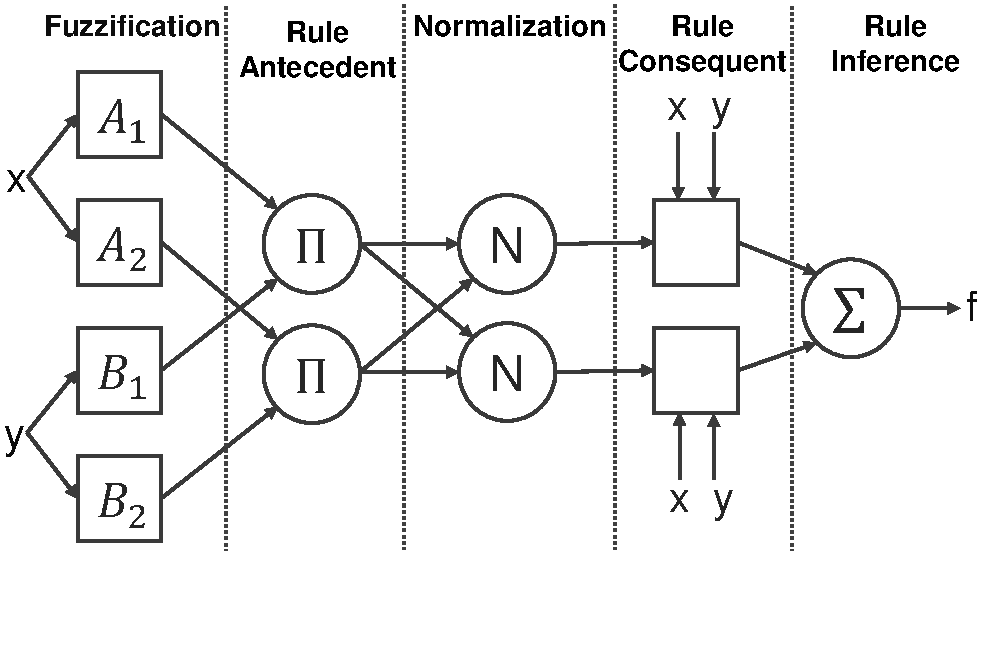
\includegraphics[width=\textwidth]{figs/Rory/ANFIS_diagram.pdf}
            \caption{}
            \label{fig:ANFIS_diagram}
          \end{subfigure}
          \hfill
          \begin{subfigure}[t]{0.48\textwidth} % Top-aligned subfigures
            \centering
            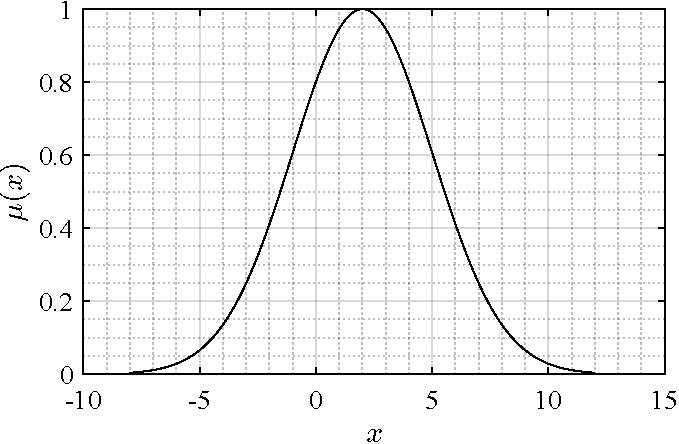
\includegraphics[width=\textwidth]{figs/Rory/mfs_plot.pdf}
            \caption{}
            \label{fig:membership_function_plot}
          \end{subfigure}
          \caption[ANFIS Network]{\textbf{a)} ANFIS network, with labelled layers. $x, \text{ } y$ represent the input, which are the $\mathcal{P}_\text{thermal},$ $\mathcal{P}_\text{radar}$, and environmental contextual data. Only two fuzzy sets and two fuzzy rules are visualised, for clarity.\textbf{b)} Gaussian membership function, with $c=2$ and $\sigma^2=9$.}
        \end{figure}

    
\subsection{ANFIS: Physics-Guided Fusion} \label{ANFIS}

    \paragraph{Membership Functions}

        A fuzzy set is a linguistic representation of a numerical variable that has been fuzzified, enabling the modelling of uncertainty and partial truth. For example, the numerical range 1-10 can be categorised into the distinct fuzzy sets \textit{high, medium, low}. The value 9 would have a high \textit{degree of membership} in the fuzzy set \textit{high}, and a low degree of membership in the other sets. Membership functions are mathematical functions that assign each input value to a degree of membership \(\in [0,1]\) for each fuzzy set. 
        
        Gaussian membership functions have been chosen to represent the all of the environmental variables, and the sensor confidence values. The Gaussian membership function is defined as
        \begin{equation}
        \label{eq:gaussian_mf}
        \mu(x) = \exp\left( -\frac{(x - c)^2}{2\sigma^2} \right),
        \end{equation}
        where \( c \) is the mode of the fuzzy set and \( \sigma^2 \) its variance, and is visualised in Figure \ref{fig:membership_function_plot}. This function is a smooth, differentiable bell curve.
        Gaussian membership functions are particularly well-suited for representing the natural variability in environmental parameters, such as soil moisture and ambient temperature, because many natural processes tend to be normally distributed, as suggested by the Central Limit Theorem \footnote{\url{https://en.wikipedia.org/wiki/Central_limit_theorem}}. Note that normalization is not necessary here because the membership values are degrees of activation rather than probability densities, and are scaled so that \(\mu(x)\in [0,1]\).
        
        In ANFIS, the network learns optimal \(c\) and \(\sigma\) parameters for each fuzzy set, tuning membership functions to best fit the fusion data. The Rule Antecedent layer determines the degree to which the fuzzy inputs satisfy the rules. The Rule Consequent layer decides the output of each rule. For Takagi-Sugeno Type-3 ANFIS \cite{jang1993anfis}, the Rule Consequents are learned as linear combinations of non-fuzzified inputs, and the outputs of all the rule consequents are combined to give a final fused confidence value. 

        
    \subsubsection{Fuzzy Rule Selection} \label{fuzzy_rules}
    

        ANFIS can be configured to include every possible 'rule' regarding the inputs to the network. However, this approach is computationally expensive, as the number of rules required scales as \((\textit{\#. fuzzy sets})^\text{(\textit{\#. inputs})}\). This makes this approach intractable when incorporating substantial domain knowledge (an example of this for time-series prediction is included in \cite{jang1993anfis}). Instead, it is more efficient to explicitly encode only the fuzzy rules that are expected to have the most significant impact, and is the approach taken here. These fuzzy rules are manually derived from the simulations in Sections \ref{compvis_thermalsims} and \ref{compvis_radarsims}, from first-principles physics, and general domain knowledge. The following rules are proposed for the ANFIS implementation:
        
        \begin{enumerate}

        
            \item \textbf{IF then soil moisture is high THEN thermal confidence is high.}

                \textbf{Justification:} As shown in Figure \ref{fig:conductivity}, the peak \(\Delta T\) increases with soil thermal conductivity. Given that soil thermal conductivity increases with soil water content \cite{wu2025soil}, and the \textbf{detectability hypothesis} in Section \ref{simulation_justification} argues that \(\Delta T\) can serve as a proxy for the detectability of a landmine viewed by the thermal sensor, it follows that higher soil moisture levels correlate with higher confidence in the thermal sensor.
            
            \item \textbf{IF soil moisture is high THEN radar confidence is low.}

                \textbf{Justification:} High soil moisture degrades radar performance by increasing the bulk soil electrical conductivity \cite{bai2013soils}, exponentially decreasing the penetration  depth\cite{giovanni2008penetration}, and thus reducing confidence in the radar sensor.

            \item \textbf{IF wind speed is high THEN thermal confidence is low}

                \textbf{Justification:} High wind speeds increase the rate of convective heat flux (Section \ref{compvis_thermalsims}) and tend to flatten soil surface temperature gradients, reducing \(\Delta T\) and thus reducing confidence in the thermal sensor.

            \item \textbf{IF soil is frozen THEN thermal confidence is low.}

                \textbf{Justification:} When the soil is frozen, any heat flow is absorbed by the latent heat of crystallisation, and temperature differences due to a landmine buried in the soil become undetectable. Therefore, thermal confidence is low when the soil is frozen.
 
        \end{enumerate}
        

        These rules are not exhaustive. If more domain knowledge becomes available, new fuzzy rules should be included to improve performance. To refine and expand the fuzzy rule database, an experimental campaign should be conducted to investigate the effects of additional environmental parameters on the sensor readings.

    
    \paragraph{Learning Approach of ANFIS}
    
        The ANFIS framework adopts a hybrid learning strategy that combines a feed-forward pass with backward error propagation. In the feed-forward phase, the fusion weightings (consequent parameters) are optimised with a least squares error (LSE) approach, whilst on the backwards pass, the membership function parameters (premise parameters) are optimised with gradient descent. This is described in Jang 1993 \cite{jang1993anfis}.
        
    
    By integrating physics-based constraints through fuzzy rules, and employing an adaptive learning strategy, ANFIS offers a fusion method that is both robust and interpretable. This approach is expected to outperform traditional methods by providing a solution grounded in the physical principles of sensor detection, as validated in Section \ref{compvis_anfisvalid}.
    